\documentclass[11pt]{article}
\usepackage[margin=1in]{geometry}
\usepackage{amsmath,amssymb,booktabs,graphicx,xcolor}
\usepackage[colorlinks=true,linkcolor=blue,citecolor=blue]{hyperref}
\title{\textsc{peaches} and \textsc{peanuts}: affine-invariant ensemble HMC\\
that scales, preconditions, and tolerates short warmup}
\author{}
\date{}

\begin{document}
\maketitle

\noindent
\textsc{peaches} (ensemble ChEES-HMC) and \textsc{peanuts} (ensemble NUTS)
are gradient-based affine-invariant ensemble samplers: a cloud of walkers
runs Hamiltonian dynamics preconditioned by the \emph{empirical covariance
of the live ensemble}, so the metric is read off the walkers each iteration
rather than fit during a separate warmup. This note isolates three clean,
reproducible properties on controlled targets (Gaussian and Rosenbrock,
exact moments known), each with seed-to-seed statistical fluctuation shown:

\begin{enumerate}
\item \textbf{Dimensional scaling.} On the isotropic Gaussian, per-gradient
efficiency follows the optimal-HMC law $\text{ESS}/\text{grad}\sim d^{-1/4}$,
\emph{exponentially} better than the $d^{-1}$ of the gradient-free affine
sampler \texttt{emcee} (\S\ref{sec:scaling}).
\item \textbf{Conditioning \emph{and} curvature.} A clean $2\times2$:
\textsc{peaches}/\textsc{peanuts} handle both, while each competitor handles
only one. On the ill-conditioned Gaussian they beat HMC/NUTS run \emph{without}
mass adaptation by up to $\sim\!6\!\times\!10^4\times$ (the ensemble preconditions for
free); on the curved Rosenbrock they stay converged while \texttt{emcee} ---
fine on the affine Gaussian --- fails to converge (\S\ref{sec:cond}).
\item \textbf{Warmup robustness.} \textsc{peaches}/\textsc{peanuts} are flat in
warmup length, whereas NUTS needs a long warmup to fit its mass matrix and is
$3$--$4$ orders less efficient at short warmup (\S\ref{sec:warmup}).
\end{enumerate}

All efficiencies are production-only ESS per target-gradient (ArviZ
rank-normalized split ESS); the gradient ensemble samplers
(\textsc{peaches}/\textsc{peanuts}) use $n_{\text{walkers}}\propto d$ for a
full-rank preconditioner --- exactly $4d$ in the Gaussian scaling sweep,
$\max(128,4d)$ in the conditioning and warmup experiments, and $256$--$512$ in
the harder Rosenbrock scaling (see Reproducibility). Bands/error bars are the
seed-to-seed spread on a fixed target.

% =====================================================================
\section{Dimensional scaling: $d^{-1/4}$ vs.\ $d^{-1}$}\label{sec:scaling}

\begin{figure}[h]
\centering
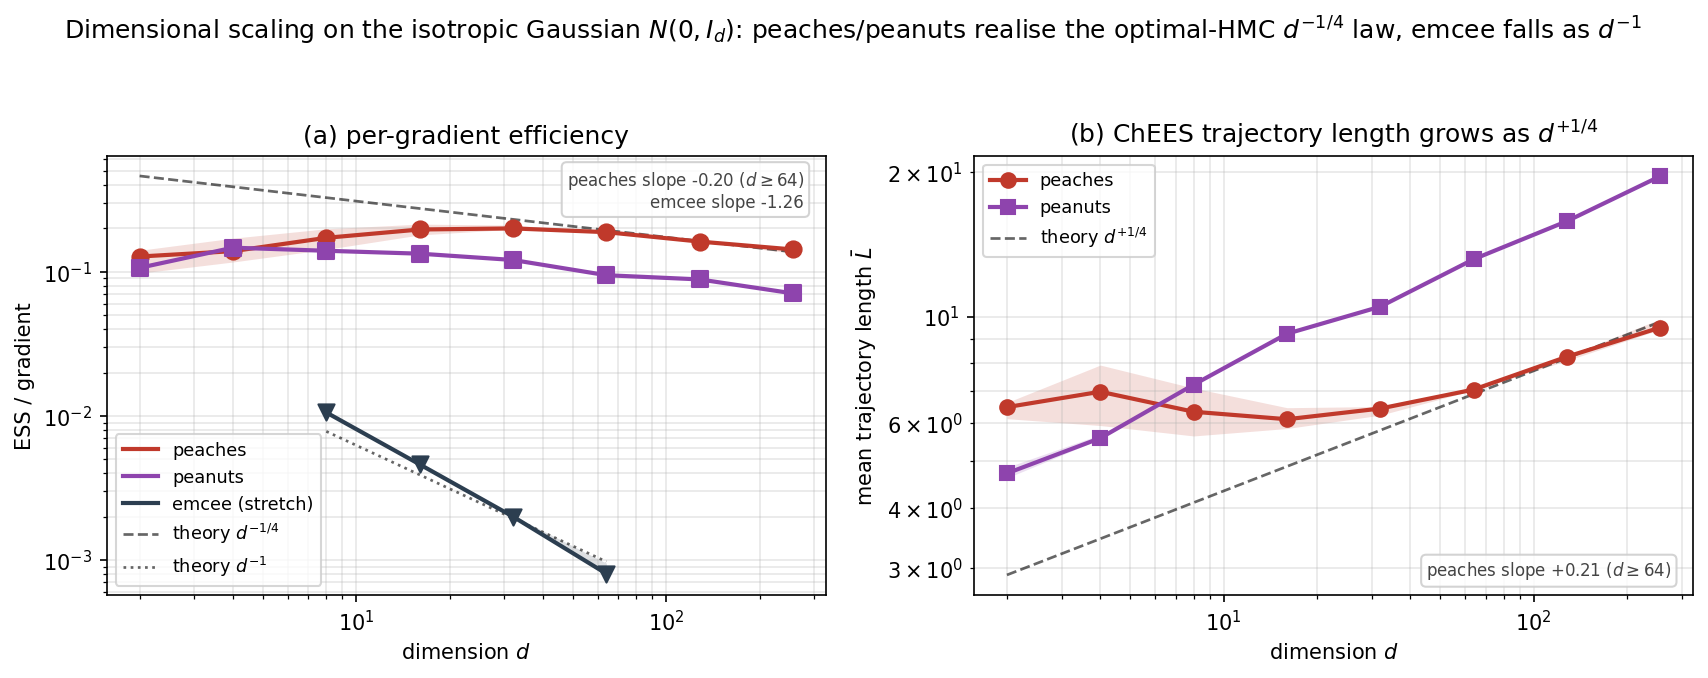
\includegraphics[width=\linewidth]{figs/pp_scaling_long.png}
\caption{Dimensional scaling on the isotropic Gaussian $N(0,I_d)$, extended down
to $d=2$ and run $10\times$ longer. Uniform protocol for the gradient samplers:
$n_{\text{walkers}}=4d$ (no floor), $\text{target\_accept}=0.8$, stretch
pre-warmup $w_s=100$, warmup $4000$, production $N=3\!\times\!10^4$ ($10^4$ at
$d{=}256$ for device memory --- per-gradient efficiency is a ratio, insensitive
to production length once converged). \texttt{emcee} uses
$n_{\text{walkers}}=\max(128,4d)$ and is run much longer (warmup
$2\!\times\!10^4$, production $10^5$) as it mixes far more slowly. Lines are the
median over the converged seeds ($6$ at $d\le16$, $3$ at $d\ge32$), bands the seed
min--max range (statistical fluctuation on a fixed target); all points converged,
rank-normalized split $\hat R\le1.03$.
\textbf{(a)} Per-gradient efficiency: \textsc{peaches}/\textsc{peanuts} approach
the optimal-HMC law $d^{-1/4}$ (dashed; fitted slope $-0.20$/$-0.21$ over
$d\in[64,256]$), while \texttt{emcee} (stretch) falls as $d^{-1}$ (dotted, slope
$-1.26$). The gentle rise for $d\lesssim16$ is pre-asymptotic --- at $4d$ walkers
the empirical ensemble covariance is noisier in few dimensions. \texttt{emcee} is
shown only to $d{=}64$; beyond that it cannot be converged in a feasible run.
\textbf{(b)} The mechanism: the ChEES-adapted mean trajectory length grows as
$d^{+1/4}$ (\textsc{peaches} slope $+0.21$), the signature of the
$\epsilon\sim d^{-1/4}$ step-size law.}
\label{fig:scaling}
\end{figure}

Optimally-tuned HMC on a $d$-dimensional product target needs a step size
$\epsilon\sim d^{-1/4}$ to hold a fixed acceptance, hence $L\sim d^{1/4}$
leapfrog steps per proposal and $\text{ESS}/\text{grad}\sim d^{-1/4}$ (Beskos
et al.\ 2013). With acceptance pinned at $0.8$ and the step size adapted, both
ensemble samplers realise this law in the asymptotic tail: over $d\in[64,256]$
the fitted efficiency slopes are $-0.20$ (\textsc{peaches}) and $-0.21$
(\textsc{peanuts}) against the theoretical $-0.25$, and the \textsc{peaches}
trajectory length grows as $d^{+0.21}$ ($\bar L: 7.1\!\to\!9.4$ as
$d:64\!\to\!256$). Below $d\sim16$ the curves are pre-asymptotic: with only $4d$
walkers the ensemble covariance is estimated from few samples, so efficiency
\emph{rises} with $d$ to a plateau near $d\sim32$ before the step-size law takes
over --- the full small-$d$ story, invisible in a high-$d$-only plot.

\texttt{emcee}'s stretch move carries no gradient information; its acceptance
and step degrade much faster with dimension, giving
$\text{ESS}/\text{grad}\sim d^{-1}$ (fitted slope $-1.26$ over the converged
$d\in[8,64]$). The gap widens exponentially in $d$: at $d{=}64$ \textsc{peaches}
is already $\sim\!235\times$ more efficient per gradient, and \texttt{emcee}
cannot be converged at all beyond $d{=}64$ in a feasible run --- itself the point.

We also examined scaling on the \emph{paired} Rosenbrock (Fig.~\ref{fig:rosen}),
formally a product of $d/2$ identical banana pairs and so in principle subject to
the same $d^{-1/4}$ law. It is not realised over the accessible range $d\le32$.
The per-block curvature gives the ChEES integrator no single good integration
length: the adapted $\bar L$ is large and \emph{bimodal} --- some seeds find the
long trajectory that traverses a banana ($\bar L\!\sim\!200$, $\mathrm{IAT}\!\sim\!1$),
others a short one ($\bar L\!\sim\!20$, $\mathrm{IAT}\!\sim\!25$) --- versus the
Gaussian's smooth $\bar L\!\sim\!6$--$9$. With enough walkers ($256$--$512$) and a
long warmup ($\ge\!12000$) \emph{every} seed converges at $d\ge8$ ($\hat R\le1.01$).
But convergence is not efficiency: a converged seed that landed in the short-$\bar L$
mode still mixes slowly ($\mathrm{IAT}\!\sim\!25$ at the same $\hat R$), so the
per-gradient efficiency is meaningful yet seed-variable --- the band reflects the
two $\bar L$ modes among the \emph{converged} seeds, not unconverged runs (at
$d{=}32$ all seeds find the long mode and the spread collapses). It stays low
($\text{ESS}/\text{grad}\!\sim\!10^{-3}$) and drifts \emph{upward} with $d$ rather
than following the law. The single/double-banana cases $d=2,4$
remain partly pathological even at $512$ walkers ($5/6$ seeds converge). The robust
statement on curvature is thus the qualitative one of \S\ref{sec:cond}:
\textsc{peaches}/\textsc{peanuts} stay efficient and converge on the banana where
\texttt{emcee} cannot --- not any clean power law.

\begin{figure}[h]
\centering
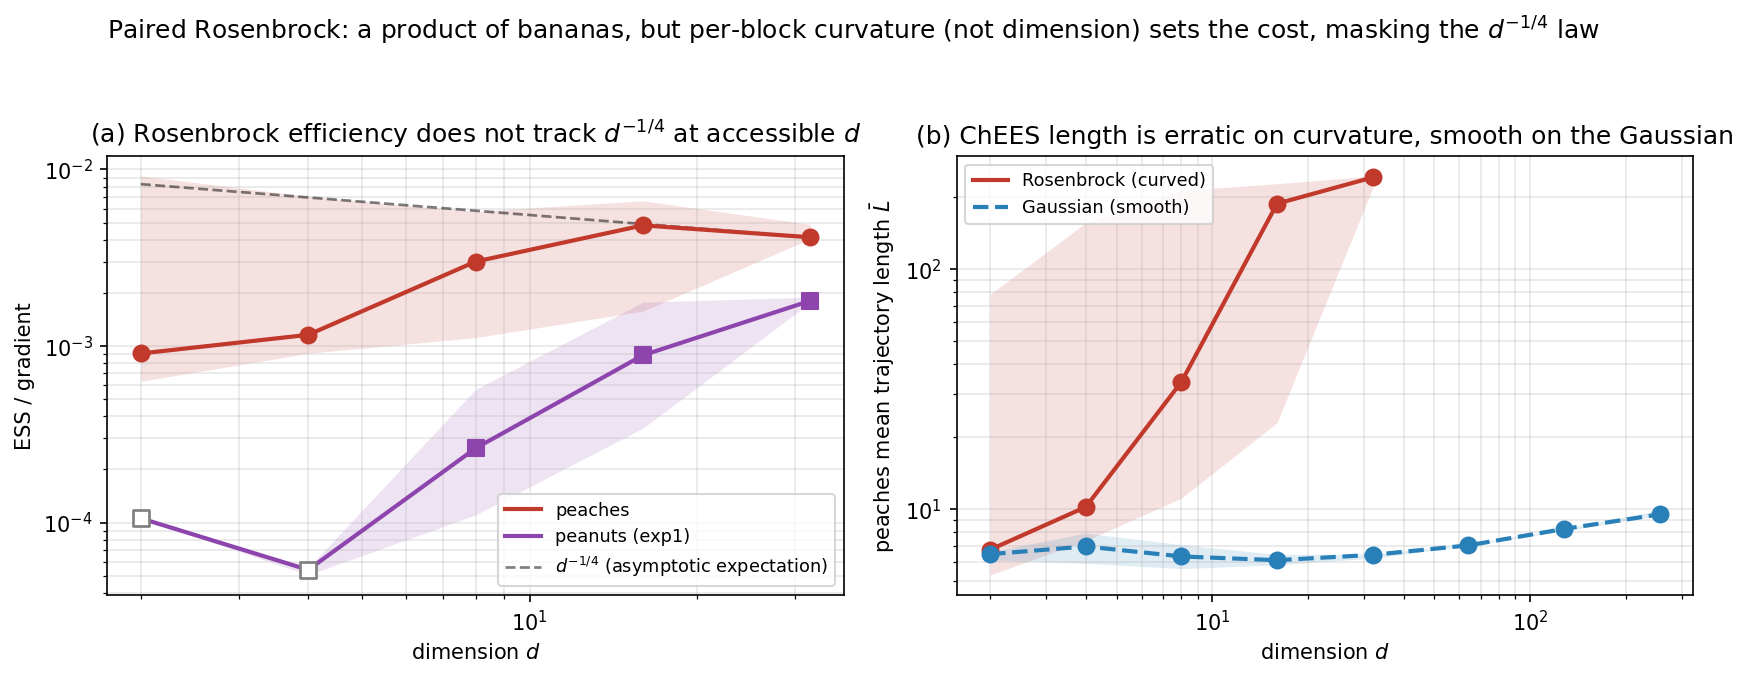
\includegraphics[width=\linewidth]{figs/pp_rosen_scaling_diag.png}
\caption{Why the paired Rosenbrock does not realise $d^{-1/4}$ over accessible
$d$, despite being a product of identical banana pairs. Median over $6$ seeds
(\textsc{peaches}, tuned runs: $256$ walkers for $d\ge8$, $512$ for $d=2,4$,
warmup $\ge\!12000$) / $3$ seeds (\texttt{peanuts}, \texttt{exp1}); band = seed
min--max over the \emph{converged} seeds only; hollow = a minority of seeds
converged. \textbf{(a)} ESS/gradient \emph{rises} with $d$ (it does not track the
$d^{-1/4}$ reference): at low $d$ the extreme single-banana curvature and the
short-$\bar L$ ChEES mode dominate. \textbf{(b)} The mechanism --- \textsc{peaches}'
adapted trajectory length is large and erratic on the curved banana
($\bar L\!\sim\!10$--$220$) but smooth and slowly-growing on the Gaussian
($\bar L\!\sim\!6$--$9$); the curvature, not the dimension, sets the cost.}
\label{fig:rosen}
\end{figure}

% =====================================================================
\section{Conditioning: the ensemble preconditions for free}\label{sec:cond}

\begin{figure}[h]
\centering
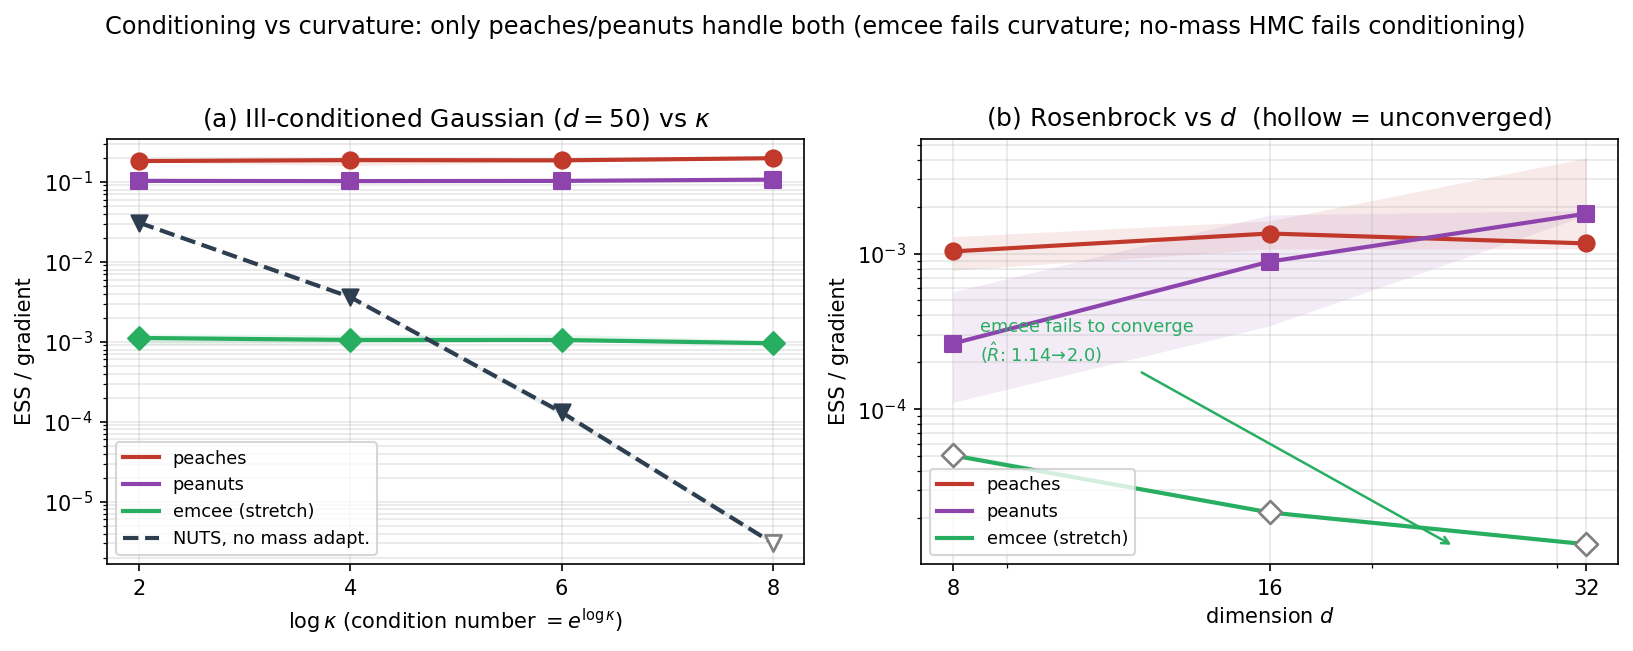
\includegraphics[width=\linewidth]{figs/pp_conditioning.png}
\caption{Robustness to conditioning and curvature. Median over $3$ seeds,
shaded bands the seed min--max range; \textbf{solid markers are converged}
($\hat R\le1.03$), \textbf{hollow are not} (their ESS\,/\,grad is not a
meaningful efficiency). Warmup/production (Gaussian\,/\,Rosenbrock):
\textsc{peaches}/\textsc{peanuts} warmup $1000$\,/\,$5000$, production
$5000$\,/\,$8000$; \texttt{emcee} warmup $1$\,/\,$2\!\times\!10^4$, production
$6$\,/\,$10\!\times\!10^4$ (run long to give it a fair chance); no-mass NUTS
$1000$/$2000$ (Gaussian). Ensemble $n_{\text{walkers}}=\max(128,4d)$, stretch
pre-warmup $w_s{=}200$\,/\,$1000$. \textbf{(a)} ill-conditioned Gaussian
($d{=}50$) vs.\ $\kappa$. \textsc{peaches}/\textsc{peanuts} and \texttt{emcee}
are flat in $\kappa$ (affine-invariant); NUTS \emph{without} mass adaptation
(identity metric) degrades sharply, collapsing and failing to converge by
$\kappa=e^8$. \textbf{(b)} Rosenbrock vs.\ dimension (peaches/peanuts vs.\ \texttt{emcee};
no-mass NUTS omitted --- it converges on Rosenbrock and is the panel-(a)
story). \textsc{peaches}/\textsc{peanuts} stay efficient and converged;
\texttt{emcee} \emph{fails to converge} for $d\!\ge\!4$ even at $10^5$ samples
(its single affine move cannot cross the curved ridge).}
\label{fig:cond}
\end{figure}

The two targets probe two \emph{different} failure modes, and the data
(Fig.~\ref{fig:cond}) gives a clean $2\times2$: \textsc{peaches}/\textsc{peanuts}
handle both; each competitor handles only one.

\paragraph{Ill-conditioned Gaussian (the \emph{conditioning} test).}
The empirical-covariance preconditioner makes
\textsc{peaches}/\textsc{peanuts} exactly affine-invariant: their ESS\,/\,grad
is flat in $\kappa$ ($\approx\!0.19$ / $\approx\!0.10$ across
$\kappa=e^{2\text{--}8}$). \texttt{emcee} is likewise $\kappa$-invariant (its
stretch move is affine), just dimensionally penalised ($\approx\!10^{-3}$ at
$d{=}50$). HMC/NUTS run with an \emph{identity} mass matrix has no such
invariance: its step size is throttled by the stiffest direction, so
ESS\,/\,grad falls from $3.1\times10^{-2}$ at $\kappa=e^2$ to
$3.0\times10^{-6}$ at $\kappa=e^8$ --- \emph{four} orders of magnitude, ending
$\sim\!6\times10^4$ below the ensemble samplers (and failing to converge,
$\hat R=1.7$, at $\kappa=e^8$). This conditioning is exactly the work NUTS
normally does in its warmup-dependent mass adaptation; the ensemble does it
for free, every iteration.

\paragraph{Rosenbrock (the \emph{curvature} test).} Here the challenge is not
global conditioning but position-dependent curvature, which no fixed linear
map can straighten. \texttt{emcee}'s single affine stretch move cannot cross
the curved ridge: even at $10^5$ samples it \emph{fails to converge} for
$d\ge\!4$ (rank-normalized split $\hat R=1.04$ at $d{=}4$, already past $1.03$,
then $1.14$, $1.40$, $2.0$ at $d{=}8,16,32$; its apparent ESS\,/\,grad is
meaningless and is greyed).
\textsc{peaches}/\textsc{peanuts} integrate \emph{local} Hamiltonian dynamics
along the ridge and stay converged and efficient
($\text{ESS}/\text{grad}\!\approx\!10^{-3}$, $\hat R\le1.03$).
No-mass NUTS, notably, \emph{does} converge here: Rosenbrock's global
conditioning is mild, so the identity metric is not the bottleneck --- which is
exactly why this panel separates the curvature failure (\texttt{emcee}) from
the conditioning failure (no-mass HMC, panel a). Only the ensemble samplers
clear both.

% =====================================================================
\section{Warmup robustness}\label{sec:warmup}

\begin{figure}[h]
\centering
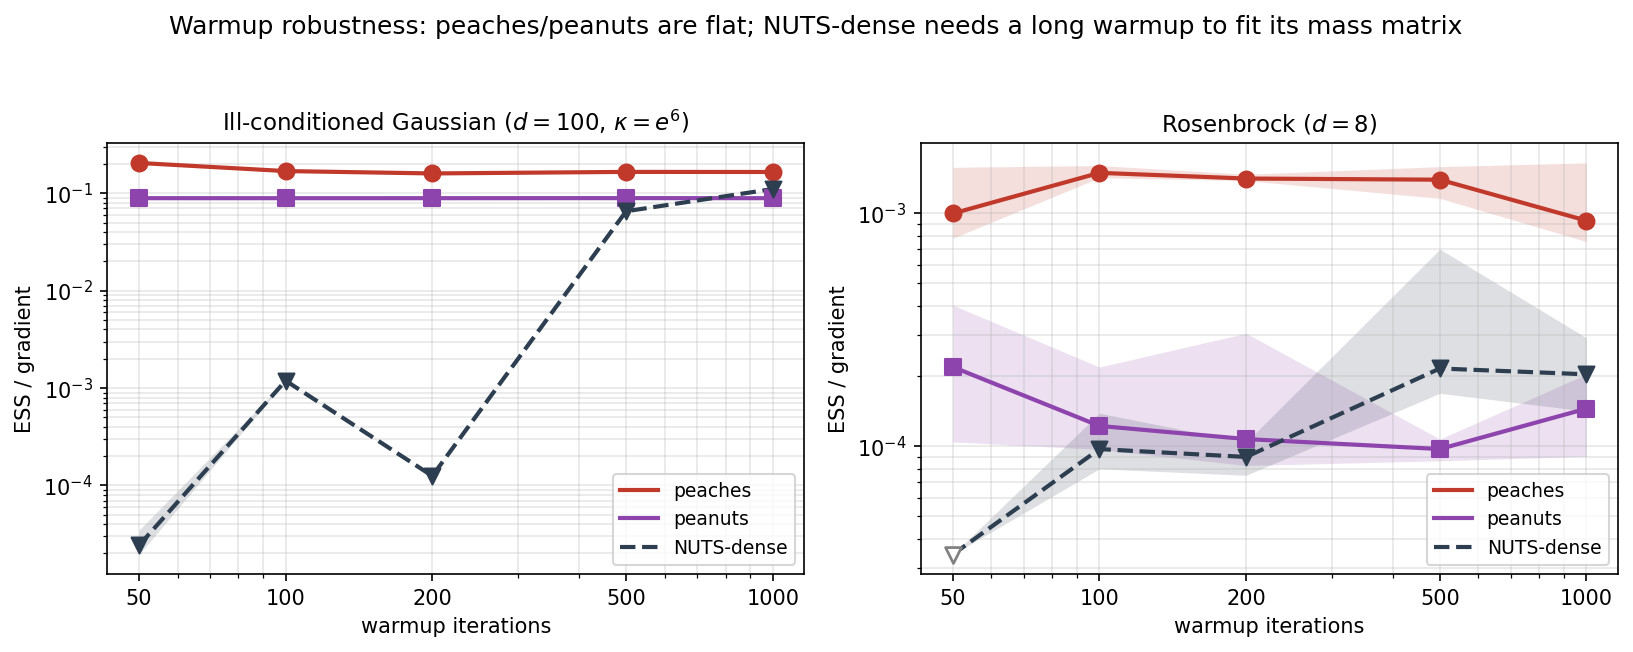
\includegraphics[width=\linewidth]{figs/pp_warmup.png}
\caption{Warmup robustness. Median over the converged seeds ($8$ sampling seeds
on a fixed target) with the band the interquartile range ($25$--$75\%$); the
Rosenbrock panel uses $256$ walkers (the Gaussian $400$), and we use the IQR
rather than min--max because ChEES's integration length is bimodal on the banana
(some seeds find the long trajectory that traverses it, others a short one ---
both converge, but min--max would span an order of magnitude). Production $5000$
samples. ESS\,/\,grad vs.\ the gradient-sampler warmup length for the
ill-conditioned Gaussian ($d{=}100$, $\kappa=e^6$) and Rosenbrock ($d{=}8$).
\textsc{peaches}/\textsc{peanuts} are flat from warmup $50$ to $1000$; NUTS-dense
needs $\gtrsim\!500$ warmup steps to fit its mass matrix and is orders of
magnitude less efficient below that.}
\label{fig:warmup}
\end{figure}

Because the preconditioner is recomputed from the live ensemble every
iteration, \textsc{peaches}/\textsc{peanuts} need no mass-matrix warmup: on the
ill-conditioned Gaussian their ESS\,/\,grad is essentially flat
($\approx\!0.16$--$0.21$ \textsc{peaches}, $\approx\!0.089$ \textsc{peanuts}) across warmup
$\in\{50,\dots,1000\}$ (Fig.~\ref{fig:warmup}, left). NUTS-dense, which must
fit a dense mass matrix during warmup, is erratic and far below at short
warmup --- $\text{ESS}/\text{grad}\approx2.4\times10^{-5}$ at warmup $50$, a factor
$\sim\!10^4$ below \textsc{peaches} --- and only becomes competitive once
warmup $\ge\!500$. The same pattern holds on Rosenbrock (right): the ensemble
samplers are warmup-insensitive while NUTS recovers only at long warmup. The
ensemble methods need only a short gradient-free stretch pre-warmup
($w_s{=}200$) to equilibrate the walker cloud's \emph{shape} --- which costs no
gradients and uses no target covariance.

% =====================================================================
\section{Reproducibility}

Targets: isotropic Gaussian $N(0,I_d)$ (scaling), ill-conditioned Gaussian
$\kappa=e^{2\text{--}8}$ rotated (conditioning/warmup), and paired Rosenbrock
(conditioning and scaling). \textsc{peanuts} uses max-tree-depth $10$; the NUTS baselines are
\texttt{numpyro} NUTS --- ``no-mass'' is \texttt{adapt\_mass\_matrix=False}
(identity metric, step size still adapted, max-tree-depth $8$) and the warmup
baseline is dense-mass. Run lengths and the stretch pre-warmup $w_s$ differ by
experiment (the samplers are robust to both, \S\ref{sec:warmup}); $3$--$6$ seeds.
Per-dimension efficiency is the median over the \emph{converged} seeds
($\hat R\le1.03$); a point is plotted solid only if a majority of its seeds
converged (hollow otherwise), and stuck seeds never enter the median. All
efficiencies are production-only ESS/grad.

\textit{Scaling} (\S\ref{sec:scaling}): isotropic $d{=}2$--$256$; gradient
samplers at uniform $n_{\text{walkers}}=4d$ (no floor), target-accept $0.8$,
$w_s{=}100$, warmup $4000$, $3\!\times\!10^4$ production ($10^4$ at $d{=}256$ for
device memory); \texttt{emcee} $n_{\text{walkers}}=\max(128,4d)$, warmup
$2\!\times\!10^4$, $10^5$ production (tags \texttt{scaleL}/\texttt{scaleLb},
\texttt{exp4c}); Gaussian low-$d$ ($d\le16$) uses $6$ seeds. The Rosenbrock
scaling (Fig.~\ref{fig:rosen}) uses \textsc{peaches} at $256$ walkers ($d\ge8$)\,/\,
$512$ ($d{=}2,4$), warmup $12000$\,/\,$15000$, target-accept $0.8$, $w_s{=}100$,
$6$ seeds (tag \texttt{scaleLd}); \texttt{peanuts} reuses \texttt{exp1}.

\textit{Conditioning} (\S\ref{sec:cond}): Gaussian $d{=}50$ vs $\kappa$ and
Rosenbrock $d\in\{8,16,32\}$; ensemble $n_{\text{walkers}}=\max(128,4d)$.
\textsc{peaches}/\textsc{peanuts} warmup $1000$\,/\,$5000$, production
$5000$\,/\,$8000$, $w_s{=}200$\,/\,$1000$ (Gaussian\,/\,Rosenbrock); \texttt{emcee}
warmup $1$--$2\!\times\!10^4$, production $6$--$10\!\times\!10^4$; no-mass NUTS
warmup $1000$, production $2000$ (tags \texttt{exp2}/\texttt{exp1},
\texttt{idmass}).

\textit{Warmup} (\S\ref{sec:warmup}): Gaussian $d{=}100$ ($\kappa=e^6$) and
Rosenbrock $d{=}8$; gradient-sampler warmup $\in\{50,100,200,500,1000\}$,
production $5000$, $w_s{=}200$, dense-mass NUTS, $8$ seeds. Gaussian
$n_{\text{walkers}}=400$ (tag \texttt{exp3}); Rosenbrock $n_{\text{walkers}}=256$
(tag \texttt{exp3b}, bumped from $128$ for cleaner short-warmup convergence).
Band is the interquartile range over converged seeds.

\section{Summary}

On controlled targets, \textsc{peaches} and \textsc{peanuts} combine the
strengths their competitors have only separately: the $d^{-1/4}$ dimensional
scaling of well-tuned HMC (\texttt{emcee} scales as $d^{-1}$), the
$\kappa$- and curvature-robustness that gradient HMC gets only \emph{with}
mass adaptation (and \texttt{emcee} gets only on affine problems), and
insensitivity to warmup length (NUTS needs a long warmup). The common cause is
the empirical-covariance ensemble preconditioner: it supplies the metric that
HMC otherwise has to learn during warmup, for free and every iteration.

\end{document}
